\section{Définition}
Une carte graphique, ou carte vidéo, est un périphérique permettant à un ordinateur de communiquer 
avec un écran.\\
\section{Fonctionnement en mode texte}
Les premières cartes graphiques datent du début des années 1980, à une époque à laquelle les ordinateurs n'affichaient que du texte à l'écran.\\
Ces cartes ne permettaient d'afficher à l'écran qu'une grille de caractères 
(25 lignes de 80 caractères) prédéfinis qui mesuraient 9x14 pixels chacun. Il était ainsi impossible de modifier directement la valeur d'un pixel.\\
Ce mode de fonctionnement ainsi que la table des caractères utilisables est 
définie par la norme MDA, "Monochrome Display Adapter"\footnote{http://www.seasip.info/VintagePC/mda.html}
du nom de la carte graphique d'IBM qui inaugura cette technologie.\\
Il est à noter que c'est le CPU\footnote{Central Processing Unit : Unité de calcul centrale / Processeur de la machine} qui donnait ses instructions à la carte graphique, celle-ci ne faisant que transmettre les caractères à l'écran.\\
Cette norme est encore utilisée de nos jours, elle permet notamment au BIOS d'afficher des informations au démarrage d'un ordinateur.
\newpage
\section{Fonctionnement en mode graphique}

En 1981 apparaît la première carte graphique permettant d'adresser chaque pixel de l'écran indépendamment.
Fabriquée par IBM, cette carte dite CGA, "Color Graphic Adapter" permettait d'utiliser une résolution de 320 par 200 pixels en mode 4 couleurs ou une résolution de 640 par 200 pixels en mode monochrome.\\
Cette carte est une avancée majeure puisqu'elle permet désormais d'afficher n'importe qu'elle forme à l'écran, et plus uniquement des caractères. C'est le début de l'informatique graphique.

\begin{center}
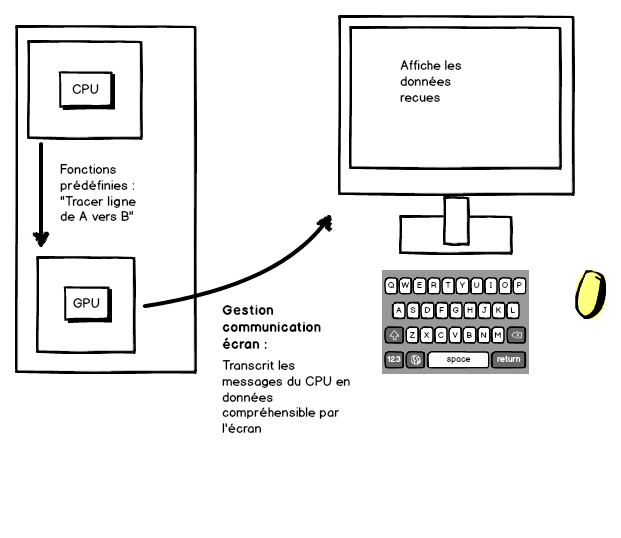
\includegraphics[width=13cm,height=8cm]{img/cpuRaster.png}

Dans ce cas le CPU va effectuer tous les calculs permettant de décomposer les formes à afficher en pixels, il les envoie ensuite à la carte graphique qui les affiche.


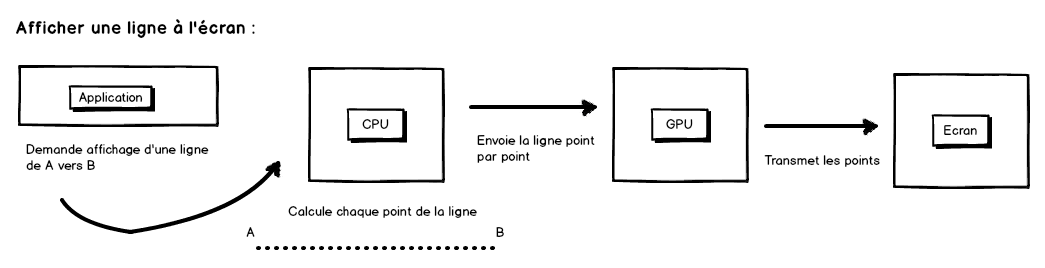
\includegraphics[width=15cm,height=6cm]{img/cpuRasterExemple.png}

Dans cet exemple c'est donc le CPU qui va effectuer la demande de l'application en décomposant la ligne en pixels qui seront envoyés à la carte graphique.\\
Ces calculs sont lourds pour le CPU, qui n'est alors composé que d'un coeur, celui ci n'est pas optimisé pour effectuer de nombreux calculs en peu de temps.

\end{center}
\newpage

\section{L'accélération matérielle 2D}

A l'époque, le rôle de la carte graphique se limitait donc à servir d'intermédiaire entre le CPU et l'écran.
\\
Aussi durant les années 1980, avec l'arrivée des interfaces graphiques, les cartes graphiques devinrent de plus en plus performantes dans le but de délester le CPU : elles étaient désormais capables de tracer elles-mêmes des primitives géométriques simples telles que des lignes, des triangles, des rectangles, des cercles, voire de colorier celles-ci d'après les consignes données par le CPU.\\

\begin{center}
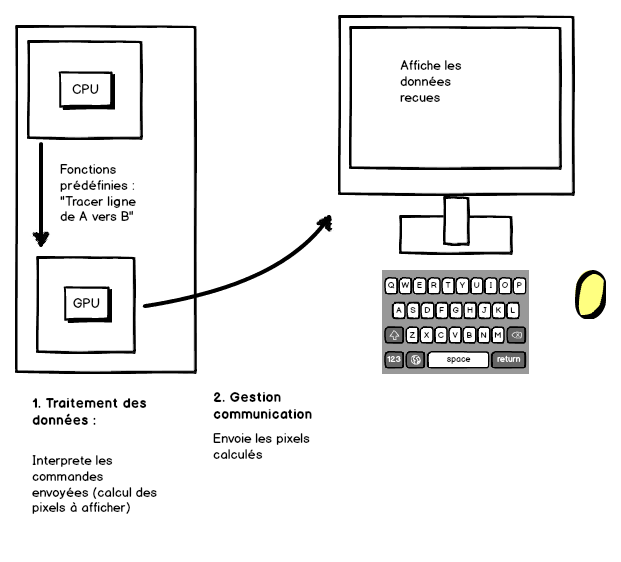
\includegraphics[width=9cm,height=8cm]{img/gpuRaster.png}

Le CPU se comporte désormais en superviseur, il demande à la carte graphique de tracer telle forme et c'est celle-ci qui effectue les calculs.


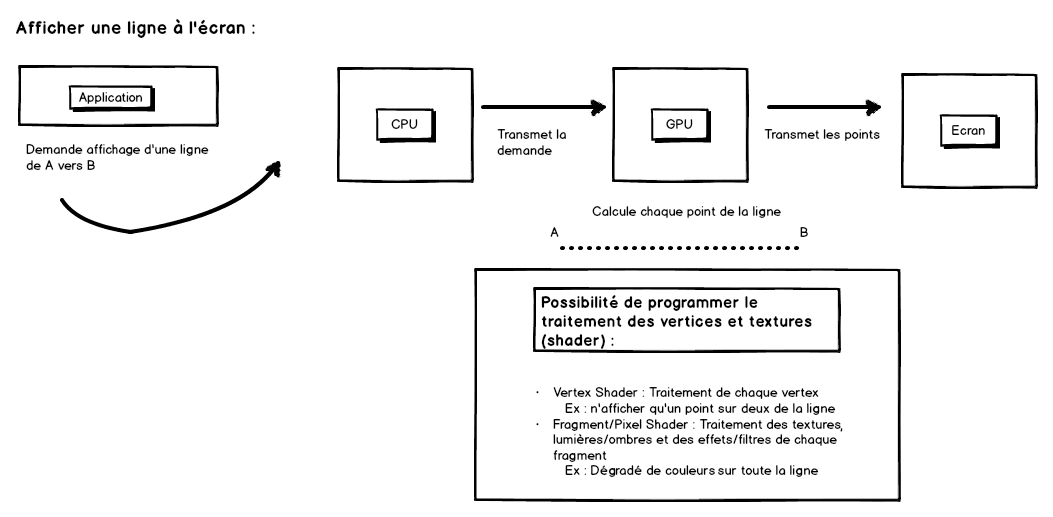
\includegraphics[width=16cm,height=6cm]{img/gpuRasterExemple.png}

Ici, c'est la carte graphique qui va calculer tous les pixels de la ligne d'après les consignes du CPU avant de les afficher à l'écran.

% Avec les cartes graphiques modernes il est maintenant possible de programmer des parties de la carte graphique appelés shader (il en existe trois : les vertex, les geometriques et les pixels ou fragments). Ceux ci peuvent permettre par exemple d'appliquer un éclairage spécifique à notre ligne.
\end{center}
\newpage

\section{L'accélération matérielle 3D}
Au début des années 1990 apparaissent les premières applications mettant en œuvre un rendu 3D. C'est notamment le jeu vidéo DOOM datant de décembre 1993 qui est considéré comme étant un pionnier en la matière.\\
L'affichage en 3D nécessite beaucoup de calculs de la part du CPU, celui-ci doit désormais calculer la projection sur l'écran de chaque point de l'espace à rendre.\\
Le constructeur 3DFX inaugure alors la première carte d'accélération 3D : la Voodoo, celle-ci permet de calculer les projections des points à la place du CPU.\\
Au fil des ans, les cartes graphiques deviennent capables d'effectuer la majeure partie des calculs nécessaires à l'affichage,  comme la gestion de l'éclairage, des ombres, l'application des textures, etc. Elles permettent
également d'accélérer le décodage de flux vidéos compressés.\\
On parle désormais de GPU, "Graphics Processing Unit" pour désigner l'unité de calcul d'une carte graphique.\footnote{A la différence du CPU, le GPU dispose d'une architecture massivement parallèle.}

\section{Différences entre GPU et CPU}

Les CPU et les GPU ont des rôles très différents.

\textbf{\\CPU} (Central Processing Unit):
\begin{itemize}
	\item	Traite l'ensemble des instructions : très polyvalent, jeu d'instructions très étendu.
	\item	Données accessibles sans contraintes.
	\item	Format de sortie libre.
	\item	Peu de cœurs, une exécution en série.
\end{itemize}

\textbf{\\GPU} (Graphics Processing Unit)
\begin{itemize}
	\item	Unités de calcul spécialisées, jeu d'instructions limité.
	\item	Grand nombre de cœurs d'exécution, architecture hautement parallèle adaptée au traitement d'images.
	\item	Format imposé en entrée et en sortie.
	\item	A pour utilité première de soulager le CPU.

\end{itemize}

De part leurs rôles différents, les CPU et les GPU ont des architectures différentes.

\newpage
\textbf{Les architectures :}
\begin{center}
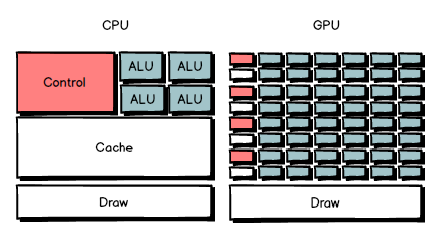
\includegraphics[width=14cm]{pipeline/images/GPUCPU.png}
\end{center}

\textbf{\\Conclusion} : Pour que l’utilisation d’un GPU soit utile et qu'il puisse mettre à profit son architecture parallèle, il faut que les calculs à effectuer soient parallèlisables.\\
C'est à dire que les calculs doivent pouvoir être répartis entre les différents coeurs d'éxécution, ce qui implique de nombreux problèmes de synchronisation et d'accès simultanés aux mêmes variables.%\footnote{ http://fr.wikipedia.org/wiki/Parall%C3%A9lisme_%28informatique%29 }



\section{Historique des cartes graphiques}
\begin{center}
\begin{tabular}{|c|c|m{0.2\linewidth}|m{0.3\linewidth} |c|}
\hline
Année & Génération & Carte & Application & Bus \\
\hline
1996 & 1 & 3dfx Voodoo & Première carte accélératrice : Texture mapping, Gestion du Z-Buffer & bus PCI\\
\hline
1998 & 2 & GeForce/ Radeon 7500 & Transform\&lighting, multi-texting & bus AGP \\
\cline{1-4}
2001 & 3 & GeForce3/ Radeon 8500 & Programmation sur les sommets (vertex shader)	& \\
\cline{1-4}
2002 & 4 & Radeon 9700/GeForce FX & Programmation sur les pixels (fragment shader)	& \\
\hline
2008 & 5 & GeForce9/ Radeon HD & Compatibilité OpenGL et DirectX,  geometry shader & bus PCIe \\
\hline
\end{tabular}
\end{center}

Source : \cite{historiqueCarte}
\\\\
Les bus PCI,(Peripheral Component Interconnect), AGP(Advanced Graphics Port) et PCIExpress sont des bus locaux
\footnote{ Bus local : système de communication entre des cartes d’extension et la carte mère}.
Le bus PCIe est une version plus petite et plus performante que le PCI et AGP.
